% CPJ application form -- compile with XeLaTeX or LuaLaTeX
\documentclass[11pt]{article}
\usepackage[a4paper,top=19.8mm,bottom=12mm,left=22.9mm,right=13.1mm]{geometry}
\usepackage{fontspec}
% Calibri throughout.
% Falls back to metric-compatible Carlito / Liberation Sans if absent.
\IfFontExistsTF{Calibri}{\setmainfont{Calibri}}{\setmainfont{Carlito}}
\usepackage[table]{xcolor}
\usepackage{array,tabularx}
\usepackage{tabularray}
\definecolor{lbl}{HTML}{F2F2F2}
\definecolor{navy}{HTML}{1F2A44}
\setlength{\parindent}{0pt}
\pagestyle{empty}
\renewcommand{\arraystretch}{1.35}
\usepackage[none]{hyphenat}
\newcolumntype{Y}{>{\raggedright\arraybackslash}X}
\newcolumntype{M}[1]{>{\raggedright\arraybackslash}m{#1}}
\newcolumntype{L}[1]{>{\raggedright\arraybackslash}p{#1}}

% Heading helpers (bold 13pt like the Word "Corps de texte" style)
\newcommand{\hone}[2]{\par\vspace{10pt}{\fontsize{13}{16}\selectfont\bfseries
  \hangindent=7.6mm\hangafter=1\makebox[7.6mm][l]{#1}#2\par}\vspace{6pt}}
\newcommand{\htwo}[2]{\par\vspace{8pt}{\fontsize{13}{16}\selectfont\bfseries\raggedright
  \leftskip=7.6mm\hangindent=9.6mm\hangafter=1\makebox[9.6mm][l]{#1}#2\par}\vspace{6pt}}
\newcommand{\note}[1]{{\fontsize{10}{12}\selectfont #1\par}}
\newcommand{\gap}[1][30pt]{\vspace{#1}}

% Extra Packages
\usepackage{wrapfig}
\usepackage{graphicx}
\usepackage[colorlinks = true,
            linkcolor = black,
            urlcolor  = black,
            citecolor = black,
            anchorcolor = black]{hyperref}
\usepackage{xurl}
\urlstyle{same}
\Urlmuskip=0mu\relax


\usepackage{etaremune}
\usepackage{enumitem}

\newcounter{descenum}
\newenvironment{descenumerate}[2]{%
  \setcounter{descenum}{#2}%
  \begin{enumerate}[
    topsep=0pt,
    itemsep=3pt,
    partopsep=0pt,
    parsep=0pt,
    label={[#1\arabic{descenum}]}
  ]
}{
  \end{enumerate}
}
\newcommand{\descitem}{%
  \item
  \addtocounter{descenum}{-1}
}
\newcommand{\bt}[1]{{\textbf{\color{teal} #1}}}
\newcommand{\boldheading}[1]{{\fontsize{13}{16}\selectfont\bfseries{#1}\vspace{6pt}}}
\setlength{\emergencystretch}{3em}

\newcommand{\update}[1]{{\color{red} #1}}

\begin{document}

\begin{center}
{\fontsize{20}{24}\selectfont\bfseries Application for a tenure-track position `junior professor'\par}
\end{center}
\vspace{6pt}

\hone{1.}{Curriculum Vitae (max 2 pages)}
\htwo{1.1.}{Personal information}

{\fontsize{10}{12}\selectfont
\begin{tblr}{width=\linewidth,hlines,vlines,colspec={Q[40mm,m,bg=lbl,font=\bfseries]X[m]},rows={ht=5.2mm}}
Last name & SINGAMANENI\\
First name & Phani Teja\\
Nationality & Indian\\
Date of birth & 09-Nov-1993\\
Highest degree obtained in higher education & PhD\\
Email & phaniteja.sp@gmail.com\\
Phone number & +33 773516971\\
Mailing address & 1 Rue de Saverne, Nancy - 54000, France\\
Professional address & Bâtiment Ada Lovelace, 615 Rue du Jardin-Botanique, 54600 Villers-lès-Nancy\\
\end{tblr}\par}

\gap[12pt]
\htwo{1.2.}{Professional experience}
\vspace{6pt}
{\fontsize{10}{12}\selectfont\renewcommand{\arraystretch}{1.1}
\begin{tabularx}{0.988\linewidth}{|L{40mm}|X|X|}
\hline \rowcolor{lbl}\bfseries Year & \bfseries Position & \bfseries Institution\\
\hline Oct 2025 - Current & Postdoc &  INRIA, Nancy\\
\hline  Mar 20223 - Sep 2025 & Postdoc & LAAS-CNRS, Toulouse\\
\hline  Jan 20223 - Feb 2023 & Research Engineer & LAAS-CNRS, Toulouse\\
\hline  Jan 2019 - Dec 2022 & PhD Student & LAAS-CNRS, Toulouse\\
\hline  Jan 2019 - Dec 2022 & PhD Student & LAAS-CNRS, Toulouse\\
\hline  Aug 2016 - Nov 2018 & Research Assistant & IIT-H, Hyderabad, India\\

\hline
\end{tabularx}\par}

\gap[18pt]
\htwo{1.3.}{Scientific experience (maximum 10 lines)}
The core of my research focuses on robot motion planning. Throughout my research career, I have worked on multiple aspects of motion planning, including path and trajectory planning, optimal trajectory generation, and high-level control. My research focuses on enabling robot autonomy through practical deployment grounded in a strong theoretical foundation. I began by building robots from scratch, then transitioned to motion planning for humanoid robots, and later to human-aware motion planning for mobile robots. My current work lies at the intersection of motion planning and human–robot interaction, with the aim of enabling robots to operate safely and effectively among humans. Below, I outline my research journey in chronological order.
\htwo{1.4.}{Keywords (maximum 5)}
\htwo{1.5.}{Major events in scientific career}
\note{List up to 5 highlights from your scientific career.}
\gap[40pt]
\htwo{1.6.}{Grants and other academic activities}
\note{Grants, funding, role as a board member, consulting, expert etc.}

\hspace*{9mm}{\fontsize{11}{13}\selectfont\bfseries 1.8 Outreach and popularising science\par}
\vspace{8pt}
\note{List the occasions/events that allowed you to disseminate your work to the general public.}
\gap[40pt]
\newpage
\hone{2.}{Research activities}
% \htwo{2.1.}{Description of scientific background, including main results (maximum 1 page)}
\htwo{2.1.}{Description of scientific background}
% \textbf{Bachelor's and Master's (2014 - 2018):} 
During my bachelor's and master's at IIIT-Hyderabad, I have worked on several kinds of robotics projects. I joined the Robotics Research Center (RRC) as an honours student and worked on the development of a stair-climbing robot as my first project. 
It involved using CAD tools like Solidworks to build and analyse the robot, quasi-static phase analysis and  prototyping the robot design~\ref{air15}, \ref{iros15}. Following this, I assisted in the development
\setlength{\columnsep}{5pt}
\begin{wrapfigure}{r}{0.26\textwidth}
\begin{minipage}{0.26\textwidth}
\centering
\vspace{-\intextsep}
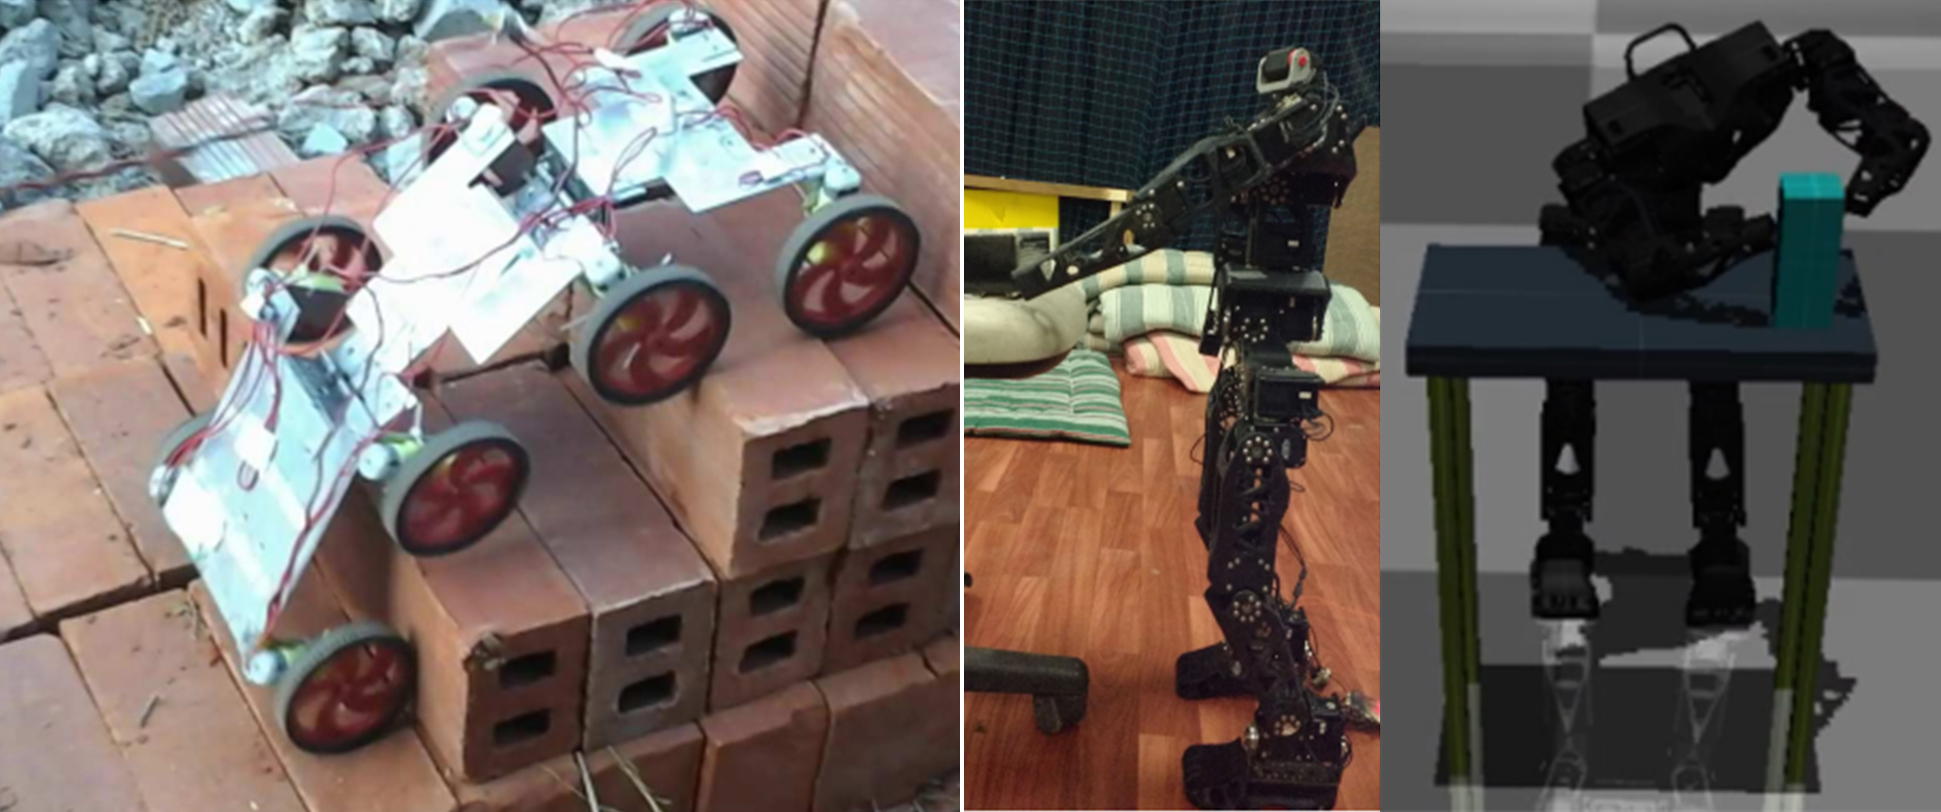
\includegraphics[width=\textwidth]{iiith2.jpg}
% \vspace{-15pt}
\end{minipage}
\begin{flushleft} 
\footnotesize 
\textit{Stair-climbing robot prototype and the 3D printed humanoid doing reachabil- ity task \ref{iros15}, \ref{robio}, \ref{humanoids18}.}
\par
\vspace{-\intextsep}
\end{flushleft}
\vspace{-\intextsep}
\end{wrapfigure}
of 3D printed humanoid robot~\ref{raha16} for building the required circuitry and system integration. In my master’s, I explored various aspects of humanoid whole-body motion planning and developed novel solutions to inverse kinematics. I proposed a reinforcement learning–based methodology for finding stable inverse kinematics configurations~\ref{robio}, which was later extended to dual-arm reachability tasks~\ref{isr18}. As part of this extension, I introduced a new reinforcement learning architecture, DiGrad~\ref{humanoids18}. Further, I completed a three-month exchange at IIT-Jodhpur under Prof. Suril Shah, where I mentored three bachelor’s students on project implementation. The project involved capturing human motion using a motion capture system and transferring these motions to a humanoid robot.

% \textbf{PhD (2019 - 2022):} 
The main objective of my doctoral thesis was to develop human-aware robotic systems and provide open-source implementations. During my PhD at LAAS-CNRS, I extensively worked on a {human-aware robot navigation stack}~\ref{cohan1}, \ref{cohan2} in ROS and made the system publicly available on GitHub. 
Over time, I iteratively extended
\setlength{\columnsep}{5pt}
\begin{wrapfigure}{l}{0.28\textwidth}
\begin{minipage}{0.28\textwidth}
\centering
\vspace{-\intextsep}
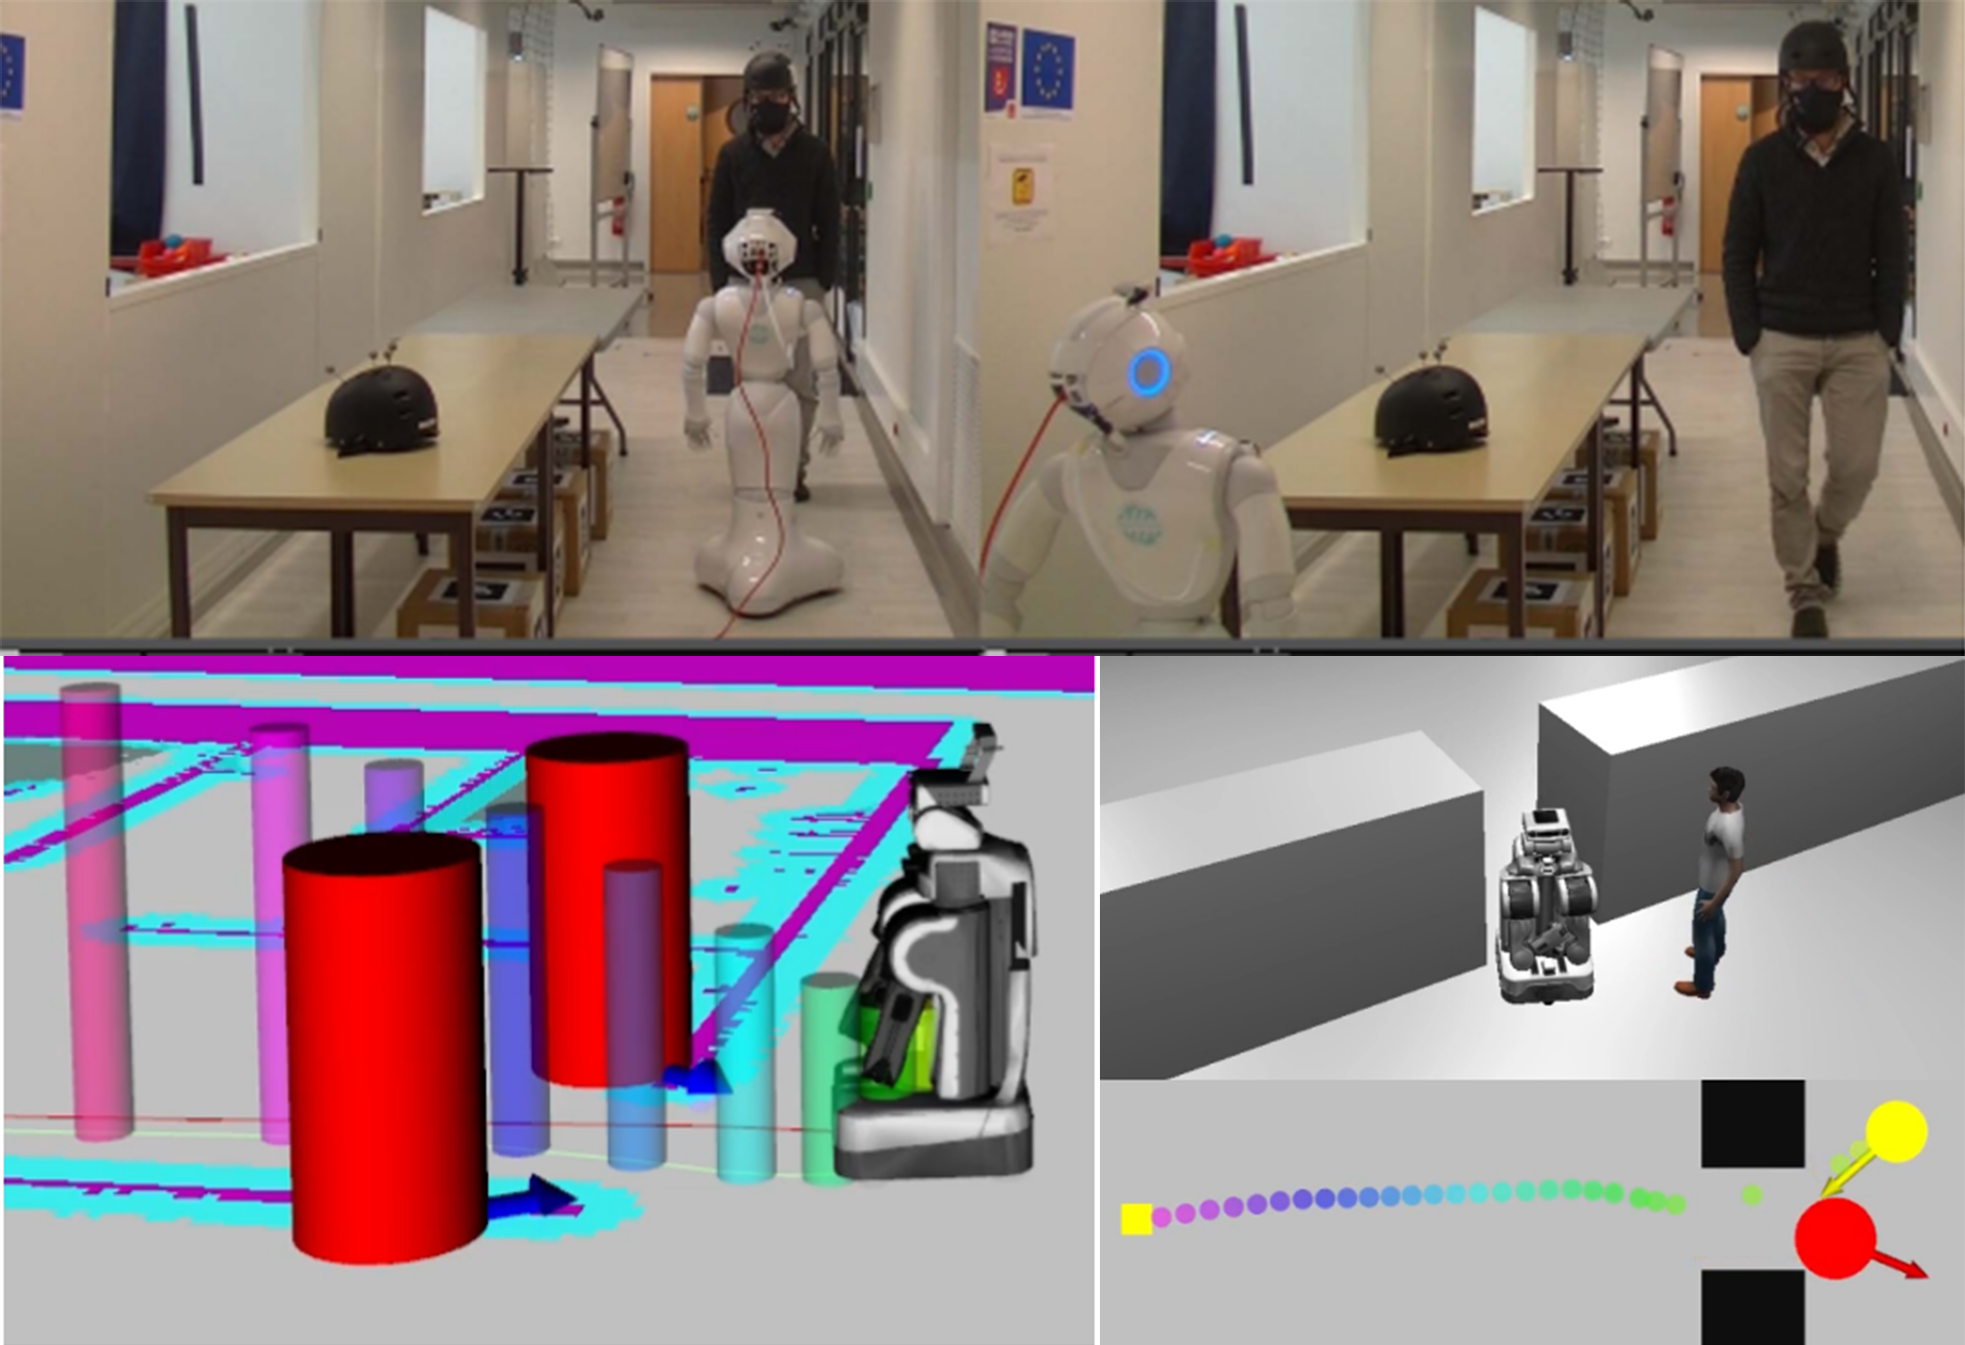
\includegraphics[width=\textwidth]{phd.jpg}
% \vspace{-\intextsep}
% \vspace{-10pt}
\end{minipage}
\begin{flushleft} 
\footnotesize 
\textit{CoHAN running on Pepper robot (top) \ref{cohan1}, \ref{cohan2}. Invisible humans in simulation (bottom left)~\ref{cohan3} and InHuS~\ref{inhus3}, \ref{inhus1}.}
\par
\vspace{-\intextsep}
\end{flushleft}
% \vspace{-\intextsep}
\end{wrapfigure}
the system with new features and implementations, including a multi-modal planning approach~\ref{cohan2}, a novel algorithm for detecting hidden humans~\ref{cohan3}, and new optimisation constraints that promote socially aware robot behaviour. The system was tested on multiple robotic platforms both at {LAAS} (PR2, Pepper and TIAGo)~\ref{cohan2}, \ref{cohan3} and at other laboratories (TIAGo, Hello Robot Stretch2, and a custom robot)~\ref{icsr24}. I also contributed to the development of intelligent human agents~\ref{inhus1}, \ref{inhus3}, \ref{imhus1} in simulation for evaluating the navigation system under diverse scenarios. As part of the {MuMMER European project}, I contributed to the development of the navigation system~\ref{mummer} for the Pepper robot during a long-term deployment at Ideapark in Tampere, Finland, and remotely supported project partners in conducting the associated long-term user study. I participated in an international social robot navigation symposium involving researchers from around the world, where we discussed key challenges and emerging research directions. This collaboration resulted in a joint article proposing {evaluation guidelines} for the field~\ref{principles}. 

\textbf{Research Enginner and Postdoc (2023 - Present)}: 
After my PhD, I worked as an engineer for two months before beginning my postdoctoral position in March at LAAS-CNRS. During this time, I focused on formalising and refining 
\setlength{\columnsep}{5pt}
\begin{wrapfigure}{r}{0.24\textwidth}
\begin{minipage}{0.24\textwidth}
\centering
\vspace{-\intextsep}
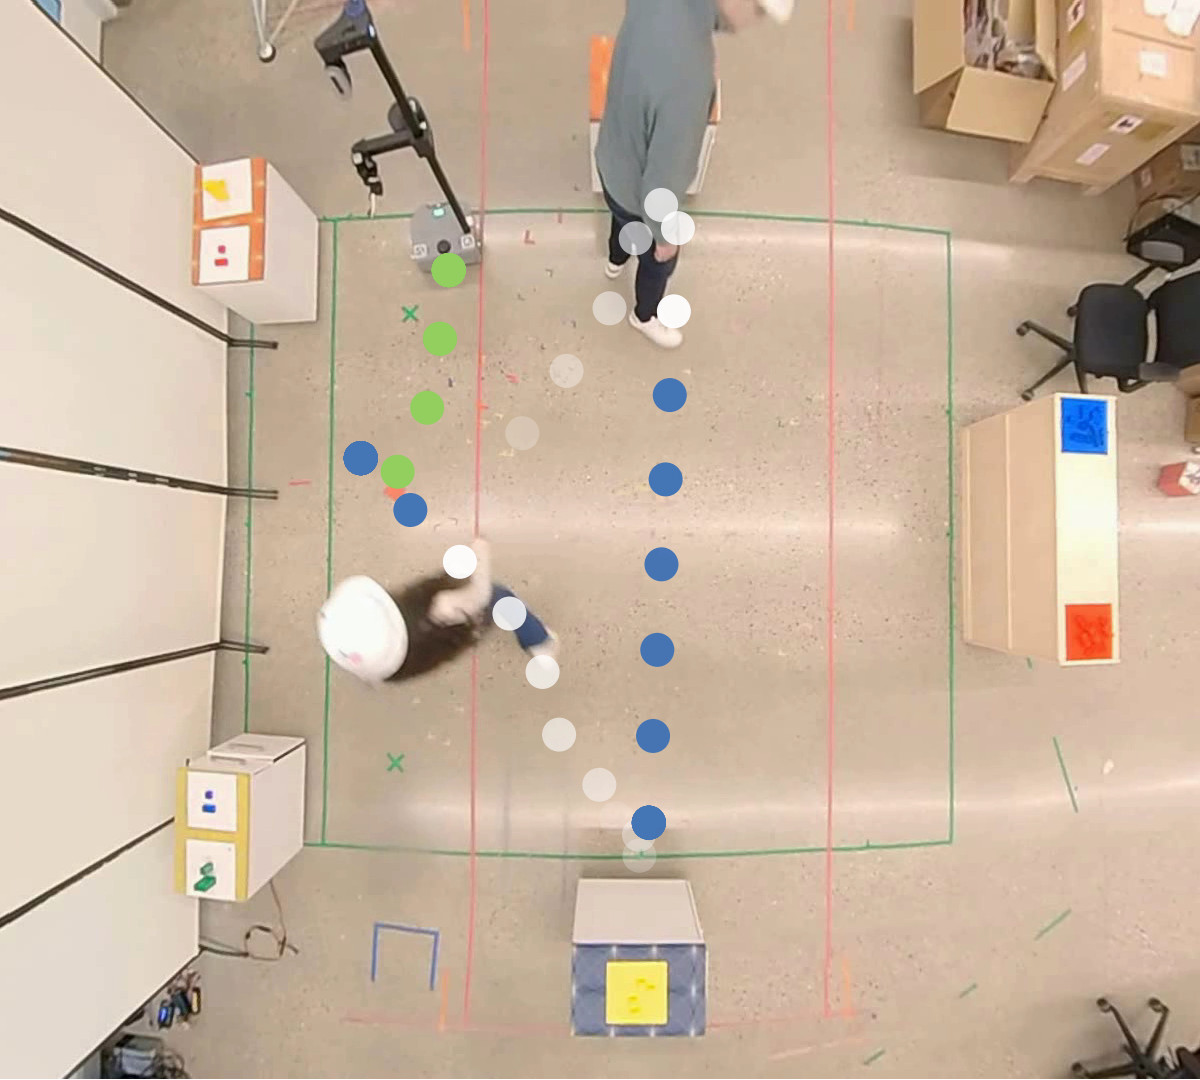
\includegraphics[width=\textwidth]{cv_frame.jpg}
\vspace{-\intextsep}
% \vspace{-10pt}
\end{minipage}
\begin{flushleft} 
\footnotesize 
\textit{Screenshot from the dataset~\ref{bi3dataset} of the user-study~\ref{hri26}.}
\par
\vspace{-\intextsep}
\end{flushleft}
\vspace{-\intextsep}
\end{wrapfigure}
a set of novel evaluation metrics~\ref{new_metrics} I had proposed at the end of my thesis. These metrics provide a better way to quantify human-aware robot navigation under different circumstances, incorporating elements such as danger and human visibility. During my postdoc at LAAS, I engaged in several collaborations while developing a new version of my human-aware robot navigation stack. This updated system incorporated new technologies, such as behaviour trees, and was made more robust. In parallel, I worked on a survey with several researchers across Europe, which was later published as a journal article~\ref{ijrr24}. I initiated a collaboration with the University of Michigan, where we conducted a dual-site user study to investigate how different motion prediction mechanisms affect user perception~\ref{bi3dataset}, \ref{hri26}. Another collaboration was conducted with researchers from CNR – Institute of Cognitive Sciences and Technologies, Rome, where we proposed a combined task and motion planning framework~\ref{icsr24}, \ref{planrob} and tested it in a simulated hospital environment.

\update{As part of the euROBIN project, I collaborated with the University of Bremen and ISIR-Paris. With Bremen, we integrated my robot navigation stack into their virtual environment, which is publicly accessible \href{https://binder.intel4coro.de/v2/gh/sphanit/cohan_multiverse_virtual_labs/HEAD}{online}
, and I also made a one-week research visit as part of this work. The collaboration with ISIR is ongoing, where we are exploring how combining LLMs and geometric reasoning can improve comfort and legibility in human-aware robot navigation. I moved to INRIA, Nancy, in October 2025, and I continue to work on the euROBIN project and socially aware robot navigation.}

\htwo{2.2.}{Scientific project for the junior professor chair (maximum 3 pages) (\textit{Research statement})}
{\itshape (Including scientific context, obstacles, indicators, dissemination of results)\par}
\gap[30pt]

\hone{3.}{Teaching activities (maximum 2 pages)}
\htwo{3.1.}{Teaching experience in higher education}
\gap[10pt]
\htwo{3.2.}{Pedagogical project related to the junior professorship within the host institution (maximum 2 pages) (\textit{Teaching statement})}
\gap[20pt]

\hone{4.}{Exhaustive list of contracts and funding obtained in research activities (if applicable)}
{\fontsize{9}{10.5}\selectfont\renewcommand{\arraystretch}{1.15}
\begin{tabularx}{0.988\linewidth}{|Y|Y|Y|Y|Y|Y|}
\hline \bfseries Year & \bfseries Source (funding body) & \bfseries Project title &
\bfseries Coordinators name & \bfseries Budget (€) & \bfseries Your role in the project\\
\hline \rule{0pt}{8mm} & & & & & \\
\hline \rule{0pt}{8mm} & & & & & \\
\hline \rule{0pt}{8mm} & & & & & \\
\hline
\end{tabularx}\par}

\hone{5.}{Comprehensive list of publications, books, patents, talks, poster presentations}
\htwo{5.1.}{Summary}
{\fontsize{10}{12}\selectfont\renewcommand{\arraystretch}{1.9}
\begin{tabularx}{\linewidth}{|L{78mm}|X|}
\hline Number of peer-reviewed articles & \\
\hline \renewcommand{\arraystretch}{1}\begin{tabular}[c]{@{}l@{}}Number of other publications (proceedings,\\ conference proceedings, book chapters, etc.)\end{tabular} & \\
\hline Number of patents & \\
\hline Number of oral communications & \\
\hline Number of poster communications & \\
\hline Number of invited seminars & \\
\hline
\end{tabularx}\par}

\gap[12pt]
\htwo{5.2.}{Peer-reviewed articles}
\begin{descenumerate}{J}{2}
    \descitem \label{principles} Anthony Francis and Claudia Pérez-D'Arpino and Chengshu Li and Fei Xia and Alexandre Alahi and Rachid Alami and Aniket Bera and Abhijat Biswas and Joydeep Biswas and Rohan Chandra and Hao-Tien Lewis Chiang and Michael Everett and Sehoon Ha and Justin Hart and Jonathan P. How and Haresh Karnan and Tsang-Wei Edward Lee and Luis J. Manso and Reuth Mirksy and Sören Pirk and \textbf{Phani Teja Singamaneni} and Peter Stone and Ada V. Taylor and Peter Trautman and Nathan Tsoi and Marynel Vázquez and Xuesu Xiao and Peng Xu and Naoki Yokoyama and Alexander Toshev and Roberto Martín-Martín. ``\textit{Principles and Guidelines for Evaluating Social Robot Navigation Algorithms}'', {ACM Transactions on Human-Robot Interaction}, 14, 2, Article 34 (June 2025), 65 pages. \url{https://doi.org/10.1145/3700599}.
    \descitem \label{ijrr24} \textbf{Phani Teja Singamaneni}, Pilar Bachiller-Burgos, Luis J. Manso, Anaís Garrell, Alberto Sanfeliu, Anne Spalanzani, Rachid Alami. ``\textit{A Survey on Socially Aware Robot Navigation: Taxonomy and Future Challenges}'', {The International Journal of Robotics Research}, 2024; 43(10), pp.1533-1572. \url{https://doi.org/10.1177/02783649241230562}.
\end{descenumerate}

\htwo{5.3.}{Other publications (proceedings, conference proceedings, book chapters, etc.)}

\boldheading{Conferences}

\begin{descenumerate}{C}{21}
    \descitem \label{hri26} Andrew Stratton , \textbf{Phani Teja Singamaneni}, Pranav Goyal, Rachid Alami, Christoforos Mavrogiannis. ``\textit{How Human Motion Prediction Quality Shapes Social Robot Navigation Performance in Constrained Spaces}'', \bt{ACM/IEEE International Conference on Human-Robot Interaction (HRI)}, 2026. (Accepted)
    
    \descitem \label{bi3dataset}  Andrew Stratton , \textbf{Phani Teja Singamaneni}, Pranav Goyal, Rachid Alami, Christoforos Mavrogiannis. ``\textit{Bi$^3$: A Biplatform, Bicultural, Biperson Dataset for Social Robot Navigation}'', \bt{International Conference on Robotics and Automation (ICRA)}, 2026. (Accepted)
    \descitem \label{rrc-irca26} Antareep Singha, Laksh Nanwani, Mathai Mathew, Samkit Jain,\textbf{ Phani Teja Singamaneni}, Arun Kumar Singh, K. Madhava Krishna. ``\textit{Crowd-FM: Learned Optimal Selection of Conditional Flow Matching-generated Trajectories for Crowd Navigation}'', \bt{International Conference on Robotics and Automation (ICRA)}, 2026. (Accepted)

    \descitem \label{icsr24} {\textbf{Phani Teja Singamaneni}, Marcello Tascioni, Alessandro Umbrico, Andrea Orlandini, and Rachid Alami. ``\textit{Contextual Social Navigation through Integrated Task and Motion Planning}'', International Conference on Social Robotics, ICSR + AI 2024. vol 15563, pp 404–416. \url{https://doi.org/10.1007/978-981-96-3525-2_34}.}

    \descitem \label{mummer} {Amandine Mayima, Guillaume Sarthou, Guilhem Buisan, \textbf{Phani Teja Singamaneni}, Yoan Sallami, Jules Waldhart, Kathleen Belhassein, Aurélie Clodic, Rachid Alami. ``\textit{How to make a robot guide?}", International Symposium on Experimental Robotics, ISER 2023. Springer Proceedings in Advanced Robotics, vol 30, pp. 483–494. \url{https://doi.org/10.1007/978-3-031-63596-0_43}.}

    \descitem \label{inhus3} {Anthony Favier, \textbf{Phani Teja Singamaneni}, Rachid Alami, ``\textit{Challenging Human-Aware Robot Navigation with an Intelligent Human Simulation System}", Social Simulation Conference, ESSA 2023. Springer Proceedings in Complexity, pp 505–518. \url{https://doi.org/10.1007/978-3-031-57785-7_39}.}

    \descitem \label{new_metrics} {\textbf{Phani Teja Singamaneni}, Anthony Favier, and Rachid Alami. ``\textit{Towards Benchmarking Human-Aware Robot Navigation: A New Perspective and Metrics}'', \bt{IEEE International Conference on Robot and Human Interactive Communication (RO-MAN)}, 2023, pp. 914-921. doi:\url{10.1109/RO-MAN57019.2023.10309398}.}
    
    \descitem \label{imhus1} {Olivier Hauterville, Camino Fernández, \textbf{Phani Teja Singamaneni}, Anthony Favier, Vicente Matellán, and Rachid Alami. ``\textit{Interactive Social Agents Simulation Tool for Designing Choreographies for Human-Robot-Interaction Research}'', ROBOT2022: Fifth Iberian Robotics Conference: Advances in Robotics, ROBOT 2022. Lecture Notes in Networks and Systems, vol 590, pp. 514–527. \url{https://doi.org/10.1007/978-3-031-21062-4_42}.}

    \descitem\label{inhus1} {Anthony Favier, \textbf{Phani Teja Singamaneni}, and Rachid Alami. ``\textit{An Intelligent Human Avatar to Debug and Challenge Human-aware Robot Navigation Systems}'', \bt{ACM/IEEE International Conference on Human-Robot Interaction (HRI)}, 2022, pp. 760-764, doi: 10.1109/HRI53351.2022.9889651.}
        
    \descitem \label{cohan3} {\textbf{Phani Teja Singamaneni}, Anthony Favier, and Rachid Alami. ``\textit{Watch out! There may be a Human. Addressing Invisible Humans in Social Navigation}'', \bt{IEEE/RSJ International Conference on Intelligent Robots and Systems (IROS)}, 2022, pp. 11344-11351, doi: \url{10.1109/IROS47612.2022.9982186}.}
    
    \descitem {Jérôme Truc, \textbf{Phani Teja Singamaneni}, Daniel Sidobre, Serena Ivaldi, and Rachid Alami. ``\textit{Khaos: a kinematic human aware optimization-based system for reactive planning of flying-coworker}'', \bt{International Conference on Robotics and Automation (ICRA)}, 2022, pp. 4764-4770, doi: \url{10.1109/ICRA46639.2022.9811803}.}
    
    \descitem \label{cohan2} {\textbf{Phani Teja Singamaneni}, Anthony Favier, and Rachid Alami. ``\textit{Human-Aware Navigation Planner for Diverse Human-Robot Interaction Contexts}'', \bt{EEE/RSJ International Conference on Intelligent Robots and Systems (IROS)}, 2021, pp. 5817-5824, doi: \url{10.1109/IROS51168.2021.9636613}.}

    \descitem \label{cohan1} {\textbf{Phani Teja S} and Rachid Alami. ``\textit{Hateb-2: Reactive planning and decision making in human-robot co-navigation}'', \bt{IEEE International Conference on Robot and Human Interactive Communication (RO-MAN)}, 2020, pp. 179-186, doi: \url{10.1109/RO-MAN47096.2020.9223463}.}

    \descitem \label{iv19} {Raghu Ram Theerthala, AVS Sai Bhargav Kumar, Mithun Babu, \textbf{S Phaniteja}, and K. Madhava Krishna. ``\textit{Motion planning framework for autonomous vehicles: A time scaled collision cone interleaved model predictive control approach}'', IEEE Intelligent Vehicles Symposium (IV), 2019, pp. 1075-1080, doi: \url{10.1109/IVS.2019.8813823}.}

    \descitem \label{meha19} {Meha Kaushik, Nirvan Singhania, \textbf{Phaniteja S} and K. Madhava Krishna. ``\textit{Parameter sharing reinforcement learning architecture for multi agent driving}'', In Proceedings of the 2019 4th International Conference on Advances in Robotics (AIR '19). Article 31, pp. 1–7. \url{https://doi.org/10.1145/3352593.3352625}.}

    \descitem \label{isr18} {\textbf{Phaniteja Singamaneni}, Parijat Dewangan, Abhishek Sarkar, and Madhava K. Krishna.``\textit{Learning Multi-Goal Inverse Kinematics in Humanoid Robot}'', ISR 2018; 50th International Symposium on Robotics, Munich, Germany, 2018, pp. 1-6.}

    \descitem \label{humanoids18} {\textbf{S Phaniteja}, Parijat Dewangan, Pooja Guhan, K. Madhava Krishna, and Abhishek Sarkar. ``\textit{Learning dual arm coordinated reachability tasks in a humanoid robot with articulated torso}'', \bt{IEEE-RAS 18th International Conference on Humanoid Robots (Humanoids)}, 2018, pp. 1-9, doi: \url{10.1109/HUMANOIDS.2018.8624979}.}

    \descitem \label{robio} {\textbf{S Phaniteja}, Parijat Dewangan, Pooja Guhan, Abhishek Sarkar, and K. Madhava Krishna. ``\textit{A deep reinforcement learning approach for dynamically stable inverse kinematics of humanoid robots}'', IEEE International Conference on Robotics and Biomimetics (ROBIO), 2017, pp. 1818-1823, doi: \url{10.1109/ROBIO.2017.8324682}.}

    \descitem \label{raha16} {Divyanshu Goel, \textbf{S Phani Teja}, Parijat Dewangan, Suril V. Shah, Abhishek Sarkar, and K. Madhava Krishna. ``\textit{Design and development of a humanoid with articulated torso}'', International Conference on Robotics and Automation for Humanitarian Applications (RAHA), 2016, pp. 1-5, doi: \url{10.1109/RAHA.2016.7931878}.}

    \descitem \label{iros15} {Sri Harsha Turlapati, Mihir Shah, \textbf{S Phani Teja}, Avinash Siravuru, and Suril V. Shah. ``\textit{Stair climbing using a compliant modular robot}'', \bt{IEEE/RSJ International Conference on Intelligent Robots and Systems (IROS)}, 2015, pp. 3332-3339, doi: \url{10.1109/IROS.2015.7353841}.}

    \descitem \label{air15} {\textbf{S Phani Teja}, Sri Harsha, Avinash Siravuru, Suril V. Shah, and K. Madhava Krishna. ``\textit{An improved compliant joint design of a modular robot for descending big obstacles}'', In Proceedings of the 2015 Conference on Advances In Robotics (AIR '15). Article 68, pp. 1–6. \url{https://doi.org/10.1145/2783449.2783518}.}
\end{descenumerate}
\vspace{6pt}

\boldheading{Workshops}
\begin{descenumerate}{W}{5}
   \descitem \label{planrob} {\textbf{Phani Teja Singamaneni}, Alessandro Umbrico, Andrea Orlandini, and Rachid Alami. ``\textit{Adaptive Robot Navigation through Integrated Task and Motion Planning}'', \bt{PlanRob Workshop, International Conference on Automated Planning and Scheduling (ICAPS)}, 2023.}

    \descitem {\textbf{Phani Teja Singamaneni}, Alessandro Umbrico, Andrea Orlandini, and Rachid Alami. ``\textit{Towards Enhancing Social Navigation through Contextual and Human-related Knowledge}'', International Conference on Social Robotics, ALTRUIST Workshop, 2022. https://hdl.handle.net/20.500.14243/515335.}

    \descitem \label{imhus2} {Olivier Hauterville, Camino Fernández, \textbf{Phani Teja Singamaneni}, Anthony Favier, Vicente Matellán, and Rachid Alami. 
    ``\textit{IMHuS: Intelligent Multi-Human Simulator}'', IEEE/RSJ International Conference on Intelligent Robots and Systems (IROS), 2022, Workshop on Artificial Intelligence for Social Robots Interacting with Humans in the Real World.}

    \descitem {\textbf{Phani Teja Singamaneni}, Anthony Favier, and Rachid Alami. ``\textit{Invisible Humans in Human-aware Robot Navigation}'', International Conference on Robotics and Automation (ICRA), 2022, Workshop on Social Robot Navigation: Advances and Evaluation.}

    \descitem \label{inhus2} {Anthony Favier, \textbf{Phani Teja Singamaneni}, and Rachid Alami. ``\textit{Simulating intelligent human agents for intricate social robot navigation}'', Robotics: Science and Systems (RSS), 2021, Workshop on Social Robot Navigation.}
 \end{descenumerate}
 
\gap[10pt]
\htwo{5.4.}{Patents}
\vspace{-6pt}{\itshape Fill in the table for each patent.\par}\vspace{6pt}
{\fontsize{10}{12}\selectfont\renewcommand{\arraystretch}{2.2}
\begin{tblr}{width=\linewidth,hlines,vlines,colspec={Q[36mm,m,bg=lbl,font=\bfseries,fg=navy]X[m]},rows={ht=7mm}}
Name & \\
Inventor(s): & \\
Patent number & \\
\end{tblr}\par}

\htwo{5.5.}{Oral communications}
\gap[40pt]
\htwo{5.6.}{Poster communications}
\gap[20pt]
\htwo{5.7.}{Invited seminars}

\end{document}
